\documentclass[12pt,a4paper]{article}
\title{Lab9-OpenCV}
\usepackage{ctex}
\usepackage{amsmath,amscd,amsbsy,amssymb,latexsym,url,bm,amsthm}
\usepackage{epsfig,graphicx,subfigure}
\usepackage{enumitem,balance}
\usepackage{wrapfig}
\usepackage{mathrsfs,euscript}
\usepackage[usenames]{xcolor}
\usepackage{hyperref}
\usepackage[vlined,ruled,commentsnumbered,linesnumbered]{algorithm2e}
\usepackage{float}
\usepackage{geometry}
\usepackage{listings}
\geometry{a4paper,scale=0.8}
\usepackage[T1]{fontenc}
\usepackage[utf8]{inputenc}
\usepackage{amssymb}
\usepackage{graphicx}
\usepackage{subfigure}
% --- Python code template ---
\usepackage[utf8]{inputenc}
% Default fixed font does not support bold face
\DeclareFixedFont{\ttb}{T1}{txtt}{bx}{n}{12} % for bold
\DeclareFixedFont{\ttm}{T1}{txtt}{m}{n}{12}  % for normal

% Custom colors
\usepackage{color}
\definecolor{deepblue}{rgb}{0,0,0.5}
\definecolor{deepred}{rgb}{0.6,0,0}
\definecolor{deepgreen}{rgb}{0,0.5,0}

\usepackage{listings}

% Python style for highlighting
\newcommand\pythonstyle{\lstset{
language=Python,
basicstyle=\ttm,
morekeywords={self},              % Add keywords here
keywordstyle=\ttb\color{deepblue},
emph={MyClass,__init__},          % Custom highlighting
emphstyle=\ttb\color{deepred},    % Custom highlighting style
stringstyle=\color{deepgreen},
frame=tb,                         % Any extra options here
showstringspaces=false
}}
% Python environment
\lstnewenvironment{python}[1][]
{
\pythonstyle
\lstset{#1}
}
{}

% Python for external files
\newcommand\pythonexternal[2][]{{
\pythonstyle
\lstinputlisting[#1]{#2}}}

% Python for inline
\newcommand\pythoninline[1]{{\pythonstyle\lstinline!#1!}}

% --- Python code template ---


% --- HTML lstlisting template --- %
\makeatletter
\usepackage{color}
\definecolor{lightgray}{rgb}{0.95, 0.95, 0.95}
\definecolor{darkgray}{rgb}{0.4, 0.4, 0.4}
%\definecolor{purple}{rgb}{0.65, 0.12, 0.82}
\definecolor{editorGray}{rgb}{0.95, 0.95, 0.95}
\definecolor{editorOcher}{rgb}{1, 0.5, 0} % #FF7F00 -> rgb(239, 169, 0)
\definecolor{editorGreen}{rgb}{0, 0.5, 0} % #007C00 -> rgb(0, 124, 0)
\definecolor{orange}{rgb}{1,0.45,0.13}		
\definecolor{olive}{rgb}{0.17,0.59,0.20}
\definecolor{brown}{rgb}{0.69,0.31,0.31}
\definecolor{purple}{rgb}{0.38,0.18,0.81}
\definecolor{lightblue}{rgb}{0.1,0.57,0.7}
\definecolor{lightred}{rgb}{1,0.4,0.5}
\usepackage{upquote}
\usepackage{listings}
% CSS
\lstdefinelanguage{CSS}{
  keywords={color,background-image:,margin,padding,font,weight,display,position,top,left,right,bottom,list,style,border,size,white,space,min,width, transition:, transform:, transition-property, transition-duration, transition-timing-function},	
  sensitive=true,
  morecomment=[l]{//},
  morecomment=[s]{/*}{*/},
  morestring=[b]',
  morestring=[b]",
  alsoletter={:},
  alsodigit={-}
}

% JavaScript
\lstdefinelanguage{JavaScript}{
  morekeywords={typeof, new, true, false, catch, function, return, null, catch, switch, var, if, in, while, do, else, case, break},
  morecomment=[s]{/*}{*/},
  morecomment=[l]//,
  morestring=[b]",
  morestring=[b]'
}

\lstdefinelanguage{HTML5}{
  language=html,
  sensitive=true,	
  alsoletter={<>=-},	
  morecomment=[s]{<!-}{-->},
  tag=[s],
  otherkeywords={
  % General
  >,
  % Standard tags
	<!DOCTYPE,
  </html, <html, <head, <title, </title, <style, </style, <link, </head, <meta, />,
	% body
	</body, <body,
	% Divs
	</div, <div, </div>, 
	% Paragraphs
	</p, <p, </p>,
	% scripts
	</script, <script,
  % More tags...
  <canvas, /canvas>, <svg, <rect, <animateTransform, </rect>, </svg>, <video, <source, <iframe, </iframe>, </video>, <image, </image>, <header, </header, <article, </article
  },
  ndkeywords={
  % General
  =,
  % HTML attributes
  charset=, src=, id=, width=, height=, style=, type=, rel=, href=,
  % SVG attributes
  fill=, attributeName=, begin=, dur=, from=, to=, poster=, controls=, x=, y=, repeatCount=, xlink:href=,
  % properties
  margin:, padding:, background-image:, border:, top:, left:, position:, width:, height:, margin-top:, margin-bottom:, font-size:, line-height:,
	% CSS3 properties
  transform:, -moz-transform:, -webkit-transform:,
  animation:, -webkit-animation:,
  transition:,  transition-duration:, transition-property:, transition-timing-function:,
  }
}

\lstdefinestyle{htmlcssjs} {%
  % General design
%  backgroundcolor=\color{editorGray},
  basicstyle={\footnotesize\ttfamily},   
  frame=b,
  % line-numbers
  xleftmargin={0.75cm},
  numbers=left,
  stepnumber=1,
  firstnumber=1,
  numberfirstline=true,	
  % Code design
  identifierstyle=\color{black},
  keywordstyle=\color{blue}\bfseries,
  ndkeywordstyle=\color{editorGreen}\bfseries,
  stringstyle=\color{editorOcher}\ttfamily,
  commentstyle=\color{brown}\ttfamily,
  % Code
  language=HTML5,
  alsolanguage=JavaScript,
  alsodigit={.:;},	
  tabsize=2,
  showtabs=false,
  showspaces=false,
  showstringspaces=false,
  extendedchars=true,
  breaklines=true,
  % German umlauts
  literate=%
  {Ö}{{\"O}}1
  {Ä}{{\"A}}1
  {Ü}{{\"U}}1
  {ß}{{\ss}}1
  {ü}{{\"u}}1
  {ä}{{\"a}}1
  {ö}{{\"o}}1
}
%
\lstdefinestyle{py} {%
language=python,
literate=%
*{0}{{{\color{lightred}0}}}1
{1}{{{\color{lightred}1}}}1
{2}{{{\color{lightred}2}}}1
{3}{{{\color{lightred}3}}}1
{4}{{{\color{lightred}4}}}1
{5}{{{\color{lightred}5}}}1
{6}{{{\color{lightred}6}}}1
{7}{{{\color{lightred}7}}}1
{8}{{{\color{lightred}8}}}1
{9}{{{\color{lightred}9}}}1,
basicstyle=\footnotesize\ttfamily, % Standardschrift
numbers=left,               % Ort der Zeilennummern
%numberstyle=\tiny,          % Stil der Zeilennummern
%stepnumber=2,               % Abstand zwischen den Zeilennummern
numbersep=5pt,              % Abstand der Nummern zum Text
tabsize=4,                  % Groesse von Tabs
extendedchars=true,         %
breaklines=true,            % Zeilen werden Umgebrochen
keywordstyle=\color{blue}\bfseries,
frame=b,
commentstyle=\color{brown}\itshape,
stringstyle=\color{editorOcher}\ttfamily, % Farbe der String
showspaces=false,           % Leerzeichen anzeigen ?
showtabs=false,             % Tabs anzeigen ?
xleftmargin=17pt,
framexleftmargin=17pt,
framexrightmargin=5pt,
framexbottommargin=4pt,
%backgroundcolor=\color{lightgray},
showstringspaces=false,      % Leerzeichen in Strings anzeigen ?
}%
%
\makeatother

%\begin{lstlisting}[style=htmlcssjs]
% --- HTML lstlisting template --- %


















\title{Lab11\quad SIFT尺度不变特征变换}
\date{2021.11}
\author{孙济宸\quad \quad 学号:520030910016 \quad  \quad 班级:F2003003}
\begin{document}
\maketitle
\section{实验概览}
按照以下步骤,实现SIFT算法,测试图像匹配效果,并与OpenCV内置库比较。
\begin{item}
\item 使用resize构建图像金字塔(5层)
\item 对于金字塔每一层图像,首先高斯模糊,去除噪声;
\item 提取特征点,原论文中使用DoG高斯差分金字塔寻找极值点,实验中采用OpenCV内置的goodFeaturesToTrack()方法直接获取特征点。
\item 计算梯度大小及方向角矩阵
\item 计算描述子。对于每个特征点,通过在

\end{item}
\section{实验环境}
\begin{itemize}
	\item OpenCV
	\item numpy

\end{itemize}
\newpage

\section{练习题的解决思路}
\begin{enumerate}


\item Gaussian模糊。用高斯算子对图片卷积,起到去除噪声的效果
\item 使用梯度算子(如Sobel)求x,y方向梯度及梯度强度。梯度算子也是对图片卷积得到梯度矩阵。用x方向、y方向的梯度算子就可以得到对应方向的梯度矩阵。 Sobel算子卷积核为:
$$s_x=
\begin{pmatrix}
 -1 & 0 & 1 \\
 -2 & 0 & 2 \\
 -1 & 0 & 1
\end{pmatrix}
$$
$$s_y=
\begin{pmatrix}
 1 & 2 & 1 \\
 0 & 0 & 0 \\
 -1 & -2 & -1
\end{pmatrix}
$$
\item 进行非极大值抑制。原理是,在一个点的梯度方向上查找,如果发现这个点不是局部最大值,则其一定不是边缘,去除之。具体操作中需要对梯度方向上的点进行插值。
\item 将上一步结果双阈值二值化。小于低限的直接置为0,大于高限的置为255,在高低限之间的看周围8邻域中有无小于高限的,有则置为255,无则置为0。
\end{enumerate}



\section{代码运行结果}

\subsection{low threshold = 40, high threshold = 100}

\begin{figure}[H]
\subfigure[原图]{
	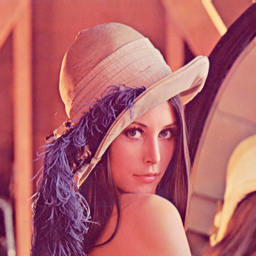
\includegraphics[width=0.5\textwidth]{1.jpg}
	\centering
}
\subfigure[自己实现Canny (Sobel)]{
	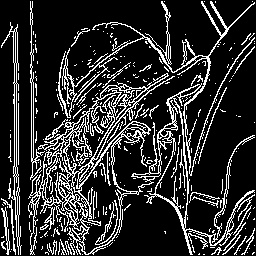
\includegraphics[width=0.5\textwidth]{./Sobel/lowTH40_hiTH100_1.jpg}
	
}
\subfigure[自己实现Canny (Prewitt)]{
	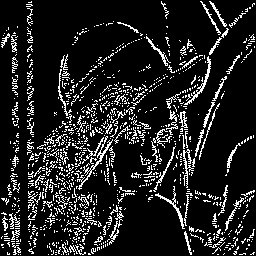
\includegraphics[width=0.5\textwidth]{./Prewitt/lowTH40_hiTH100_1.jpg}
	
}
\subfigure[cv2内置Canny]{
	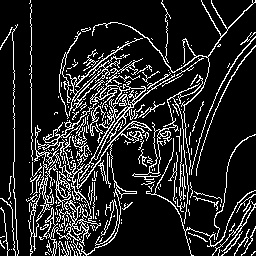
\includegraphics[width=0.5\textwidth]{./builtin/lowTH40_hiTH100_builtin_1.jpg}
	
}	
\caption{1.jpg}
\end{figure}


\begin{figure}[H]
\subfigure[原图]{
	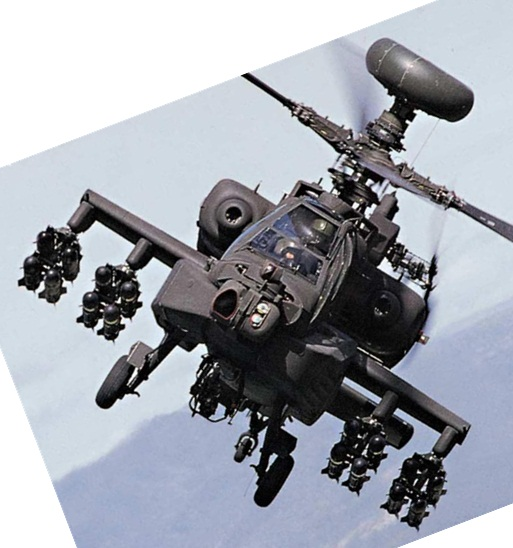
\includegraphics[width=0.5\textwidth]{2.jpg}
	\centering
}
\subfigure[自己实现Canny (Sobel)]{
	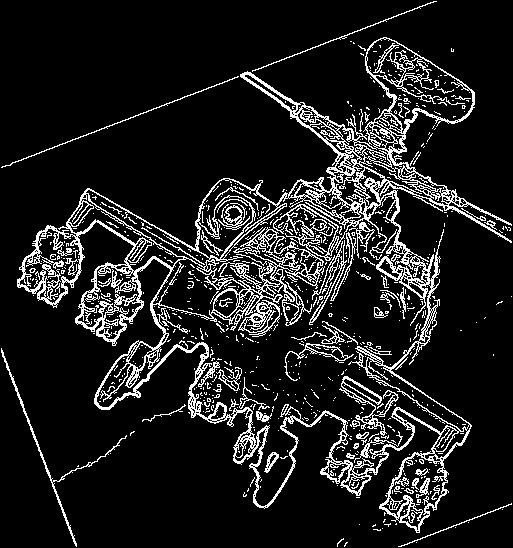
\includegraphics[width=0.5\textwidth]{./Sobel/lowTH40_hiTH100_2.jpg}
	
}
\subfigure[自己实现Canny (Prewitt)]{
	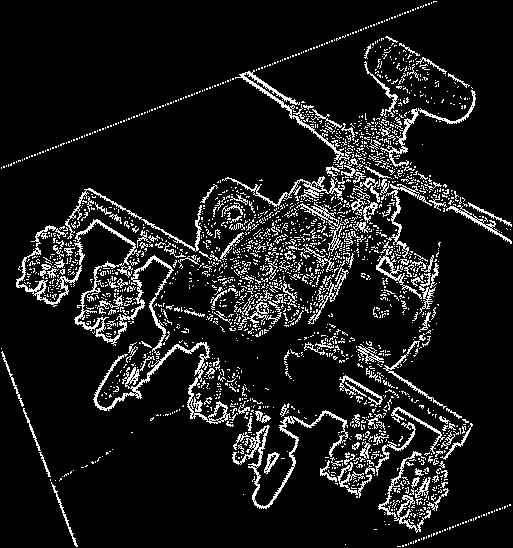
\includegraphics[width=0.5\textwidth]{./Prewitt/lowTH40_hiTH100_2.jpg}
	
}
\subfigure[cv2内置Canny]{
	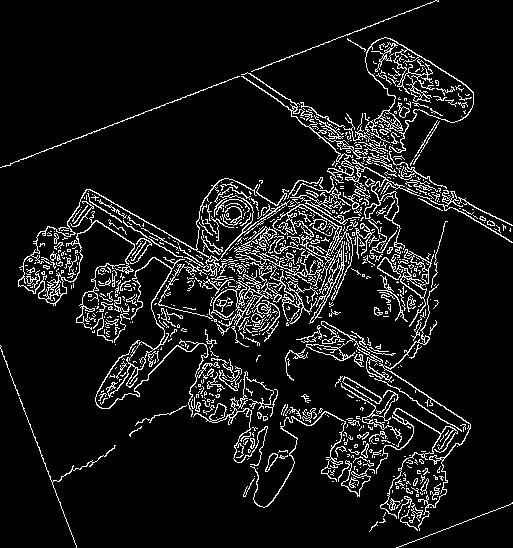
\includegraphics[width=0.5\textwidth]{./builtin/lowTH40_hiTH100_builtin_2.jpg}
	
}	
\caption{2.jpg}
\end{figure}


\begin{figure}[H]
\subfigure[原图]{
	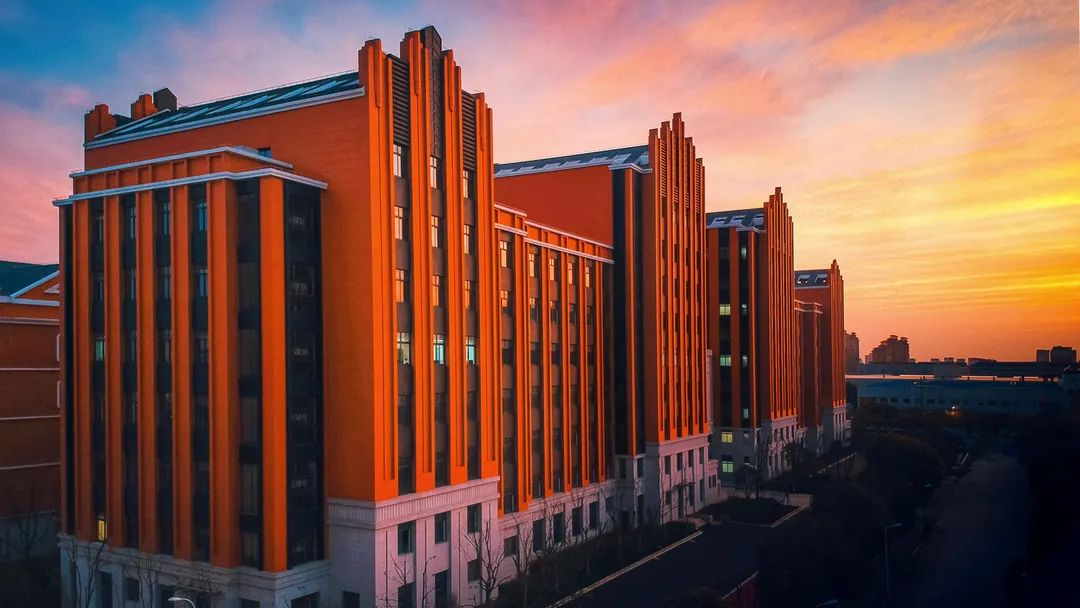
\includegraphics[width=0.5\textwidth]{3.jpg}
	\centering
}
\subfigure[自己实现Canny (Sobel)]{
	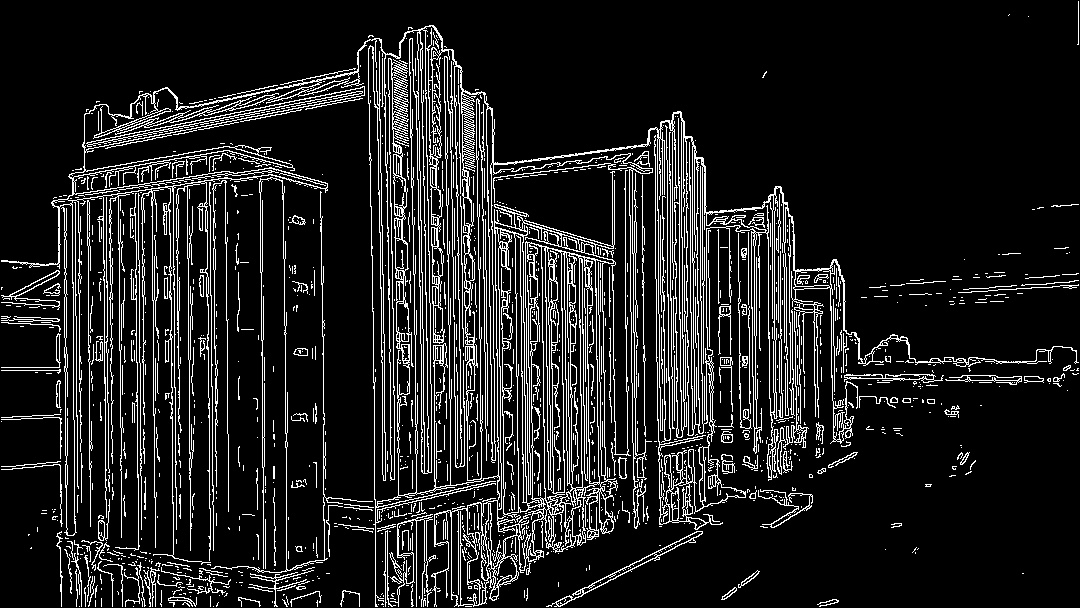
\includegraphics[width=0.5\textwidth]{./Sobel/lowTH40_hiTH100_3.jpg}
	
}
\subfigure[自己实现Canny (Prewitt)]{
	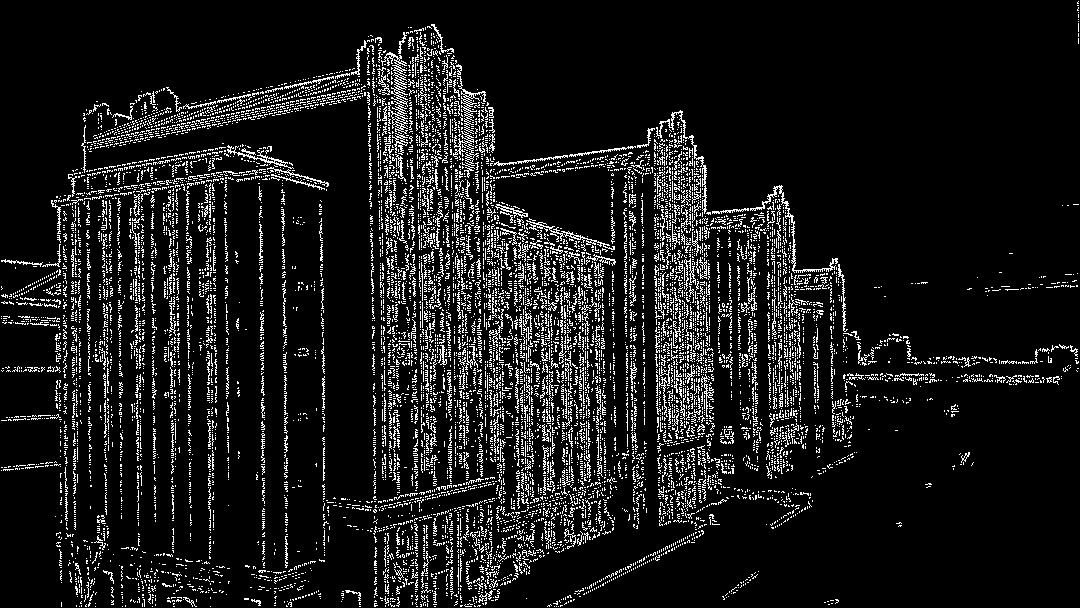
\includegraphics[width=0.5\textwidth]{./Prewitt/lowTH40_hiTH100_3.jpg}
	
}
\subfigure[cv2内置Canny]{
	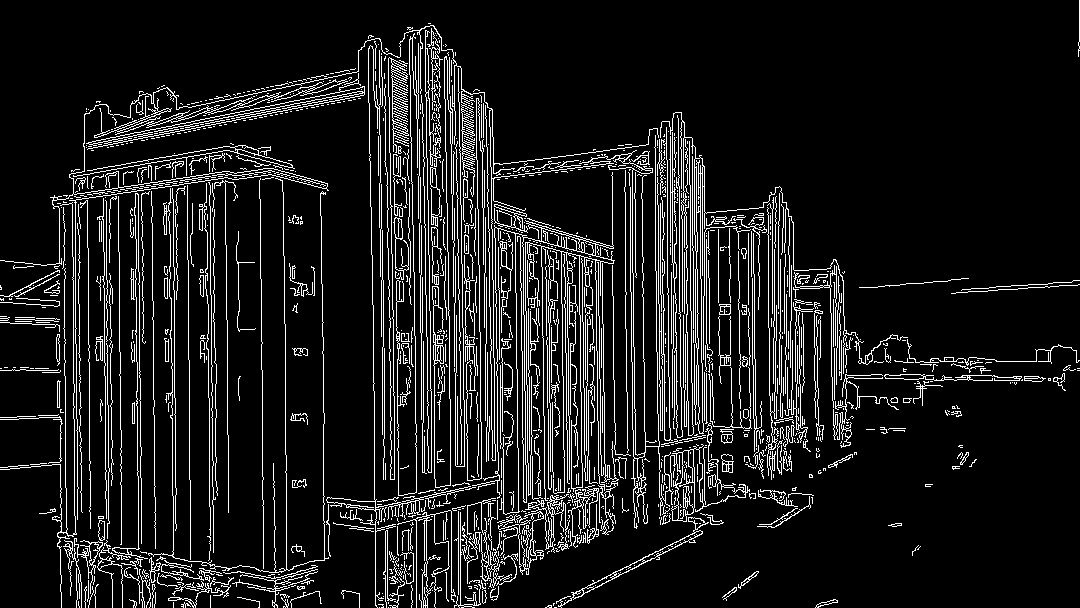
\includegraphics[width=0.5\textwidth]{./builtin/lowTH40_hiTH100_builtin_3.jpg}
	
}	
\caption{3.jpg}
\end{figure}




\subsection{low threshold = 60, high threshold = 120}



\begin{figure}[H]
\subfigure[原图]{
	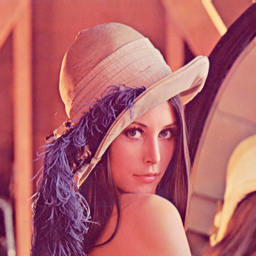
\includegraphics[width=0.5\textwidth]{1.jpg}
	\centering
}
\subfigure[自己实现Canny (Sobel)]{
	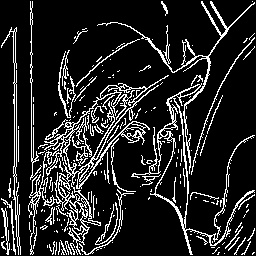
\includegraphics[width=0.5\textwidth]{./Sobel/lowTH60_hiTH120_1.jpg}
	
}
\subfigure[自己实现Canny (Prewitt)]{
	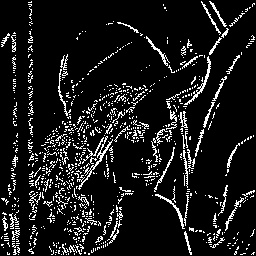
\includegraphics[width=0.5\textwidth]{./Prewitt/lowTH60_hiTH120_1.jpg}
	
}
\subfigure[cv2内置Canny]{
	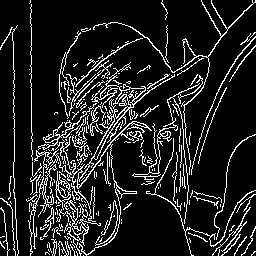
\includegraphics[width=0.5\textwidth]{./builtin/lowTH60_hiTH120_builtin_1.jpg}
	
}	
\caption{1.jpg}
\end{figure}


\begin{figure}[H]
\subfigure[原图]{
	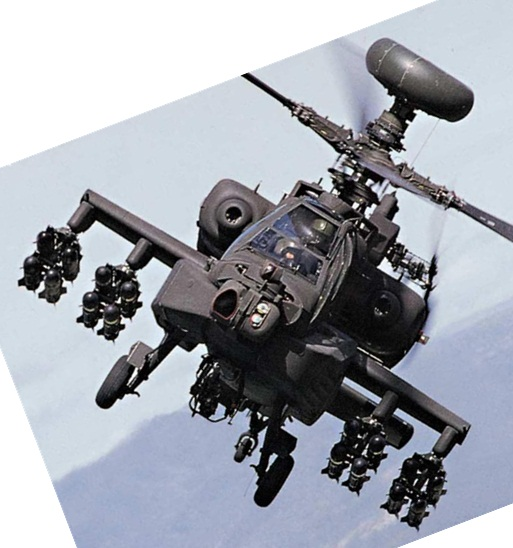
\includegraphics[width=0.5\textwidth]{2.jpg}
	\centering
}
\subfigure[自己实现Canny (Sobel)]{
	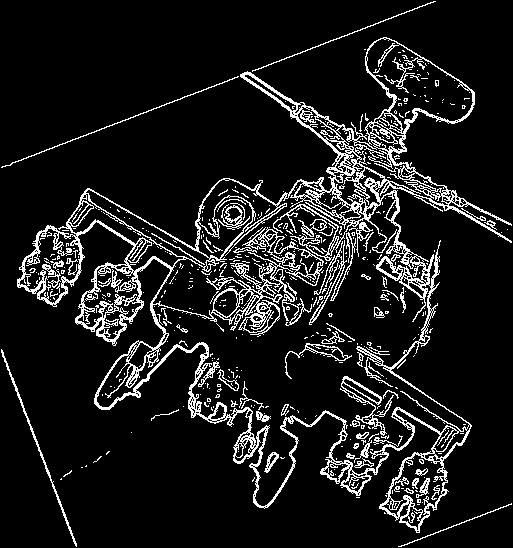
\includegraphics[width=0.5\textwidth]{./Sobel/lowTH60_hiTH120_2.jpg}
	
}
\subfigure[自己实现Canny (Prewitt)]{
	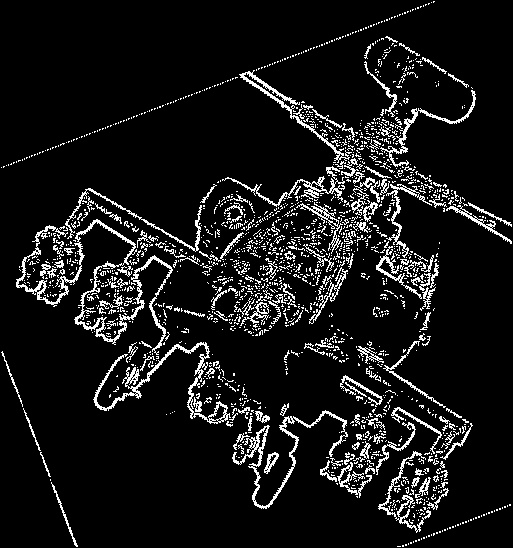
\includegraphics[width=0.5\textwidth]{./Prewitt/lowTH60_hiTH120_2.jpg}
	
}
\subfigure[cv2内置Canny]{
	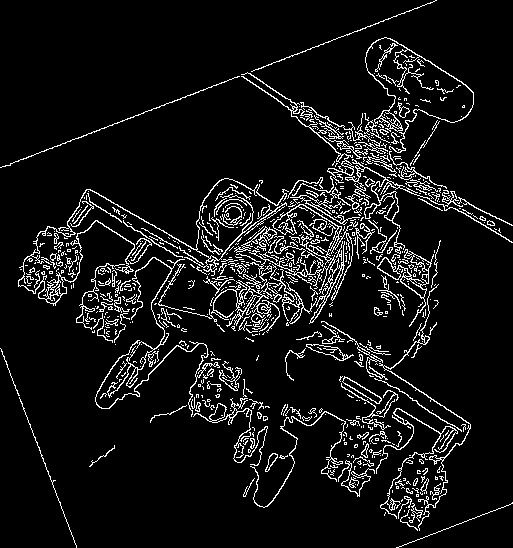
\includegraphics[width=0.5\textwidth]{./builtin/lowTH60_hiTH120_builtin_2.jpg}
	
}	
\caption{2.jpg}
\end{figure}


\begin{figure}[H]
\subfigure[原图]{
	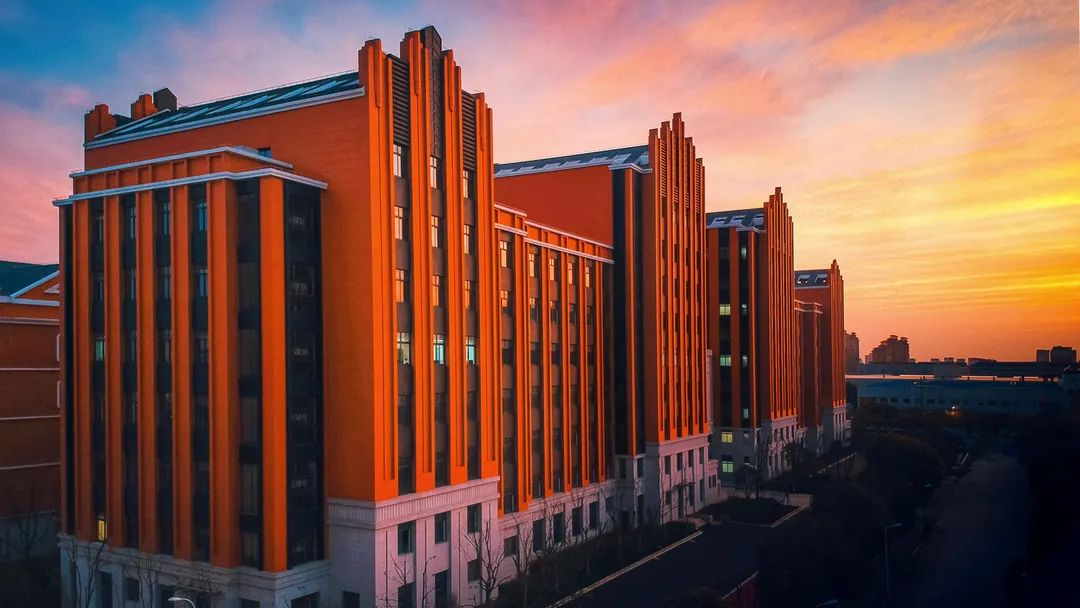
\includegraphics[width=0.5\textwidth]{3.jpg}
	\centering
}
\subfigure[自己实现Canny (Sobel)]{
	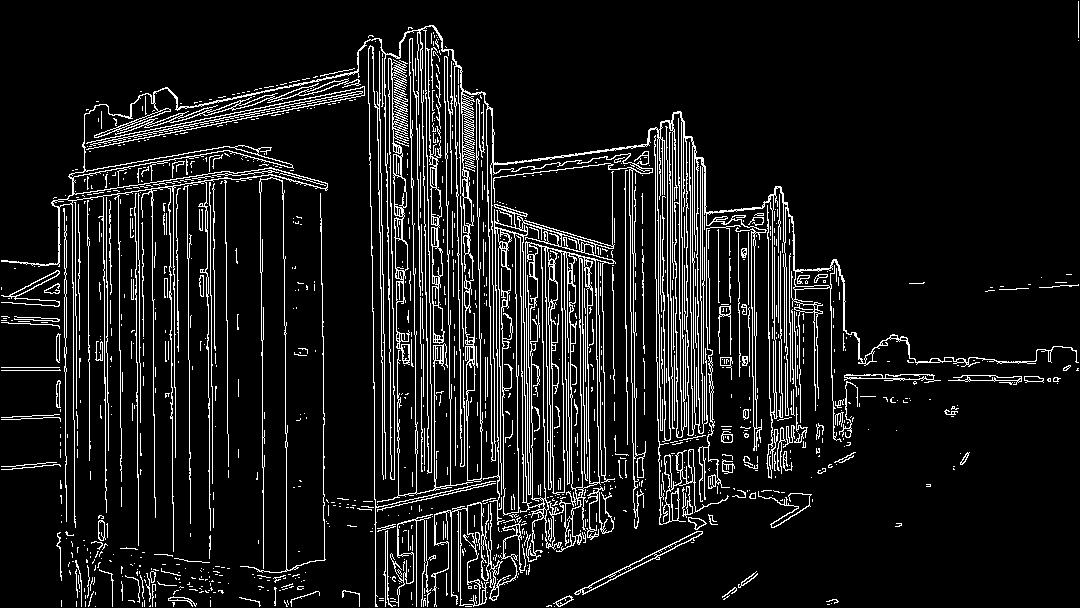
\includegraphics[width=0.5\textwidth]{./Sobel/lowTH60_hiTH120_3.jpg}
	
}
\subfigure[自己实现Canny (Prewitt)]{
	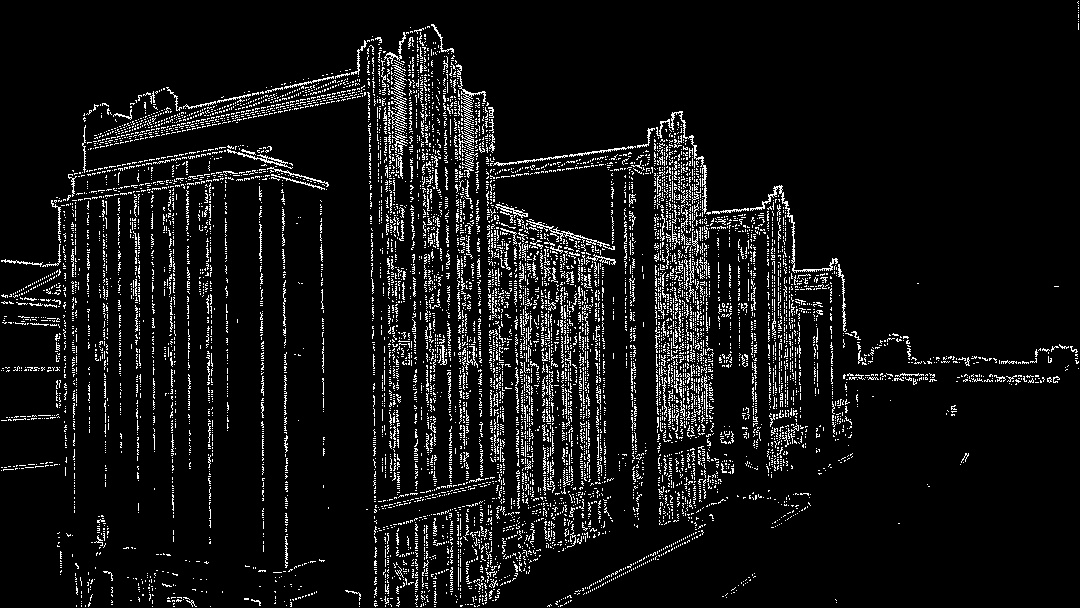
\includegraphics[width=0.5\textwidth]{./Prewitt/lowTH60_hiTH120_3.jpg}
	
}
\subfigure[cv2内置Canny]{
	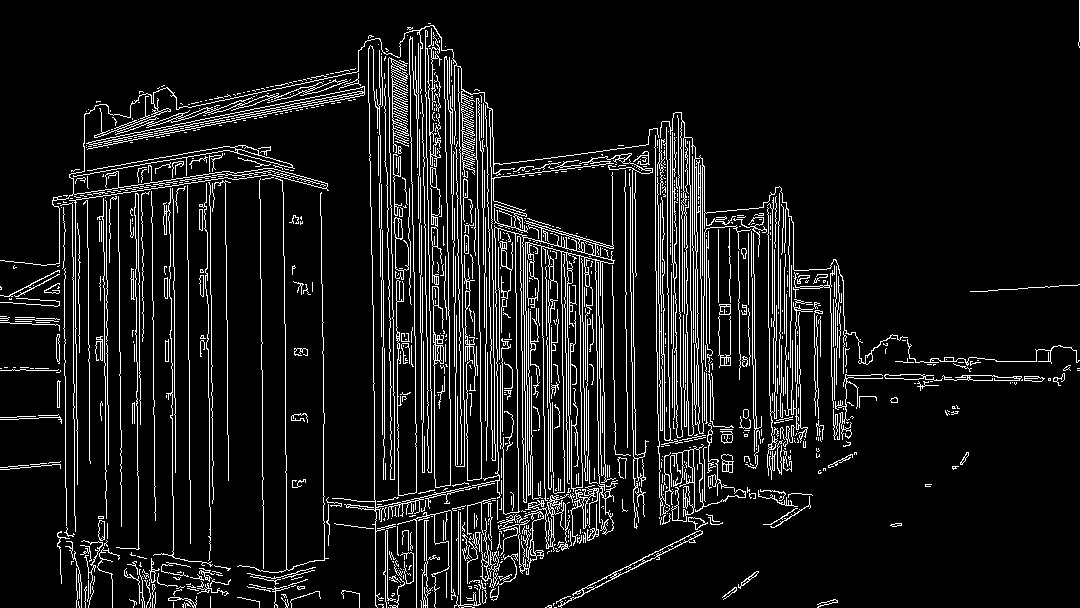
\includegraphics[width=0.5\textwidth]{./builtin/lowTH60_hiTH120_builtin_3.jpg}
	
}	
\caption{3.jpg}
\end{figure}

\section{分析与思考}
\begin{itemize}
\item 总的来说使用Sobel算子的效果是比较好的,最终实现效果接近于opencv内置的Canny算法,只是有些图片会出现较粗边缘或者双边缘,目前没有找到原因,推测可能是非极大值抑制实现方式不同。 
\item 低限和高限设置方面,设置得低可以提高边缘检测敏感度,但也对噪声更加敏感;设高了反之,能抑制噪声,但微小细节会丢失。具体使用中还是要视情况而定。
\item Prewitt算子对Canny算法效果不佳,边缘断断续续,应该是因为缺乏对与相邻像素的加权(sobel算子中是2倍)导致边缘没法很好的用双阈值法区分出来。
\item 可能是实现语言关系,自己在python中实现的Canny性能不如C语言实现的cv2库,运行速度比内置函数慢不少。
\end{itemize}

\newpage

\section{附录:python代码}
\begin{lstlisting}[style=py]
import cv2
from cv2 import Sobel, cv2 # make vscode not complain
from matplotlib import pyplot as plt
import math
import numpy as np
import copy
def combine_grad(sx, sy):
    if sx.shape != sy.shape:
        raise ValueError 
    HEIGHT, WIDTH = sx.shape[0], sx.shape[1]
    grad_M = np.zeros([HEIGHT,WIDTH])
    print(grad_M.shape)
    for i in range(HEIGHT):
        for j in range(WIDTH):
            dx, dy= float(sx[i][j]), float(sy[i][j])
            grad_M[i][j] = np.sqrt(dx * dx + dy * dy)
    
    #grad_M = grad_M * 255 / np.max(grad_M)
    return grad_M

def nonMaxSuppression(img,dx,dy):
    M = copy.deepcopy(img)
    if not (M.shape == dx.shape and M.shape == dy.shape):
        raise ValueError 
    HEIGHT, WIDTH = M.shape[0], M.shape[1]
    EPS = 1e-6
    for i in range(1, HEIGHT - 1):
        for j in range(1, WIDTH - 1):
            gradx = float(dx[i][j])
            grady = float(dy[i][j])
            if np.abs(gradx) < EPS:
                gradx = EPS
            if np.abs(grady) < EPS:
                grady = EPS
                
            #gradm = M[i][j]
            if np.abs(grady) > np.abs(gradx):  # 梯度绝对值y方向大于x方向
                w = np.abs(gradx) / np.abs(grady)
                g2 = M[i-1][j]
                g4 = M[i+1][j]
                
                if gradx * grady > 0: # x,y梯度同号
                    g1 = M[i-1][j-1]
                    g3 = M[i+1][j+1]
                else: # x,y梯度反号
                    g1 = M[i-1][j+1]
                    g3 = M[i+1][j-1]
            else:
                w =  np.abs(grady) / np.abs(gradx)
                g2 = M[i][j-1]
                g4 = M[i][j+1]
                
                if gradx * grady > 0: # x,y梯度同号
                    g1 = M[i-1][j-1]
                    g3 = M[i+1][j+1]
                else: # x,y梯度反向
                    g1 = M[i-1][j+1]
                    g3 = M[i+1][j-1]
            
            gtmp1 = w * g1 + (1 - w) * g2
            gtmp2 = w * g3 + (1 - w) * g4
            if M[i][j] < gtmp1 or M[i][j] < gtmp2:
                M[i][j] = 0

    return M

def doubleThresh(M,low_th,hi_th):
    HEIGHT, WIDTH = M.shape[0], M.shape[1]
    img = np.zeros([HEIGHT,WIDTH])
    for i in range(1, HEIGHT - 1):
        for j in range(1, WIDTH - 1):
            if M[i][j] < low_th:
                img[i][j] = 0
            elif M[i][j] > hi_th:
                img[i][j] = 255
            elif (M[i-1][j-1:j+1] < hi_th).any() or (M[i+1][j-1:j+1] < hi_th).any() or (M[i][j-1] < hi_th) or (M[i][j+1] < hi_th): # 8邻域中有小于hi_th的点
                img[i][j] = 255
    return img

def docanny(filename,method):
    SAVEDIR = 'result/' + method + '/'
    READDIR = 'dataset/'
    lo_th, hi_th = 40,100

    img_gray = cv2.imread(READDIR + filename, cv2.IMREAD_GRAYSCALE)
    img_gauss= cv2.GaussianBlur(img_gray,(3,3),0)
    if method == "Sobel":
    #Sobel
        sx = cv2.Sobel(img_gauss, cv2.CV_16S, 1, 0)  # x方向梯度
        sy = cv2.Sobel(img_gauss, cv2.CV_16S, 0, 1)  # y方向梯度
    
    if method == "Prewitt":

        kernelx = np.array([[1,1,1],[0,0,0],[-1,-1,-1]],dtype=int)
        kernely = np.array([[-1,0,1],[-1,0,1],[-1,0,1]],dtype=int)

        sx = cv2.filter2D(img_gauss, cv2.CV_16S, kernelx)
        sy = cv2.filter2D(img_gauss, cv2.CV_16S, kernely)
       
    
    M = cv2.convertScaleAbs(combine_grad(sx, sy))
    #print(M)
    img_sup = nonMaxSuppression(M, sx, sy)
    
    #cv2.imshow(filename, M)
    #cv2.waitKey(0)
    #cv2.destroyAllWindows()
    
    img_fin = doubleThresh(img_sup, lo_th, hi_th)

    cv2.imwrite(f"{SAVEDIR}/lowTH{lo_th}_hiTH{hi_th}_{filename}", img_fin)
 

def docanny_builtin(filename):
    SAVEDIR = 'result/builtin/'
    READDIR = 'dataset/'
    lo_th, hi_th = 40,100
    img_gray = cv2.imread(READDIR + filename, cv2.IMREAD_GRAYSCALE)
    img_fin = cv2.Canny(img_gray, lo_th, hi_th)
    cv2.imwrite(f"{SAVEDIR}/lowTH{lo_th}_hiTH{hi_th}_builtin_{filename}", img_fin)

if __name__ == '__main__':
    files = [
    '1.jpg',
    '2.jpg',
    '3.jpg'
    ] 
    for file in files:
        docanny(file,method="Sobel")  
        docanny(file,method="Prewitt")  
        docanny_builtin(file)




\end{lstlisting}
\end{document}



